\documentclass[a4paper, 14pt]{extarticle}

% Поля
%--------------------------------------
\usepackage{geometry}
\geometry{a4paper,tmargin=2cm,bmargin=2cm,lmargin=3cm,rmargin=1cm}
%--------------------------------------


%Russian-specific packages
%--------------------------------------
\usepackage[T2A]{fontenc}
\usepackage[utf8]{inputenc}
\usepackage[english, main=russian]{babel}

%--------------------------------------

\usepackage{textcomp}

% Красная строка
%--------------------------------------
\usepackage{indentfirst}               
%--------------------------------------             


%Graphics
%--------------------------------------
\usepackage{graphicx}
\graphicspath{ {./images/} }
\usepackage{float}%"Плавающие" картинки
%--------------------------------------

% Полуторный интервал
%--------------------------------------
\linespread{1.3}                    
%--------------------------------------

%Выравнивание и переносы
%--------------------------------------
% Избавляемся от переполнений
\sloppy
% Запрещаем разрыв страницы после первой строки абзаца
\clubpenalty=10000
% Запрещаем разрыв страницы после последней строки абзаца
\widowpenalty=10000
%--------------------------------------

%Списки
\usepackage{enumitem}

%Подписи
\usepackage{caption} 

%Гиперссылки
% \usepackage{hyperref}

\usepackage[colorlinks, urlcolor = blue, filecolor = blue, citecolor = blue, linkcolor = black]{hyperref}


\hypersetup {
unicode=true
}

%Рисунки
%--------------------------------------
\DeclareCaptionLabelSeparator*{emdash}{~--- }
\captionsetup[figure]{labelsep=emdash,font=onehalfspacing,position=bottom}
%--------------------------------------

\usepackage{tempora}

%Листинги
%--------------------------------------
\usepackage{listings} % Пакет для отображения кода
\usepackage{xcolor} % Пакет для цветных элементов

\lstset{inputencoding=utf8, extendedchars=false, keepspaces = true}

\definecolor{codegreen}{rgb}{0,0.6,0}
\definecolor{codegray}{rgb}{0.5,0.5,0.5}
\definecolor{codepurple}{rgb}{0.68,0.8,0.82}
\definecolor{backcolour}{rgb}{0.9,0.9,0.9} 
\definecolor{keyword}{rgb}{0.93, 0.68, 0.18}   % Оранжевые ключевые слова

\lstdefinestyle{mystyle}{
    backgroundcolor=\color{backcolour},   % цвет фона
    commentstyle=\color{codegreen},       % цвет комментариев
    keywordstyle=\color{keyword},        % цвет ключевых слов
    numberstyle=\tiny\color{codegray},    % стиль нумерации строк
    stringstyle=\color{codegreen},       % цвет строк
    basicstyle=\ttfamily\footnotesize,    % основной стиль текста
    breakatwhitespace=false,              % перенос по пробелам
    breaklines=true,                      % автоматический перенос строк
    captionpos=b,                         % позиция заголовка внизу
    keepspaces=true,                      % сохранять пробелы
    numbers=left,                         % нумерация строк слева
    numbersep=5pt,                        % отступ нумерации
    showspaces=false,                     % скрывать пробелы
    showstringspaces=false,               % скрывать пробелы в строках
    showtabs=false,                       % скрывать табуляцию
    tabsize=2                             % размер табуляции
}

\lstset{style=mystyle, inputencoding=utf8}



%--------------------------------------

%%% Математические пакеты %%%
%--------------------------------------
\usepackage{amsthm,amsfonts,amsmath,amssymb,amscd}  % Математические дополнения от AMS
\usepackage{mathtools}                              % Добавляет окружение multlined
\usepackage[perpage]{footmisc}


% графики
\usepackage{booktabs}        % Пакет для улучшенных таблиц
\usepackage{pgfplots}        % Пакет для построения графиков
\pgfplotsset{compat=1.17}    % Установка совместимости

% Литература 

% переименовываем  список литературы в "список используемой литературы"
\addto\captionsrussian{\def\refname{Список литературы}}






%--------------------------------------

%--------------------------------------
%			НАЧАЛО ДОКУМЕНТА
%--------------------------------------

\begin{document}

%--------------------------------------
%			ТИТУЛЬНЫЙ ЛИСТ
%--------------------------------------
\begin{titlepage}
\thispagestyle{empty}
\newpage


%Шапка титульного листа
%--------------------------------------
\vspace*{-60pt}
\hspace{-65pt}
\begin{minipage}{0.3\textwidth}
\hspace*{-20pt}\centering

\includegraphics[width=\textwidth]{emblem}
\end{minipage}
\begin{minipage}{0.67\textwidth}\small \textbf{
\vspace*{-0.7ex}
\hspace*{-6pt}\centerline{Министерство науки и высшего образования Российской Федерации}
\vspace*{-0.7ex}
\centerline{Федеральное государственное автономное образовательное учреждение }
\vspace*{-0.7ex}
\centerline{высшего образования}
\vspace*{-0.7ex}
\centerline{<<Московский государственный технический университет}
\vspace*{-0.7ex}
\centerline{имени Н.Э. Баумана}
\vspace*{-0.7ex}
\centerline{(национальный исследовательский университет)>>}
\vspace*{-0.7ex}
\centerline{(МГТУ им. Н.Э. Баумана)}}
\end{minipage}
%--------------------------------------

%Полосы
%--------------------------------------
\vspace{-25pt}
\hspace{-35pt}\rule{\textwidth}{2.3pt}

\vspace*{-20.3pt}
\hspace{-35pt}\rule{\textwidth}{0.4pt}
%--------------------------------------

\vspace{1.5ex}
\hspace{-35pt} \noindent \small ФАКУЛЬТЕТ\hspace{80pt} <<Информатика и системы управления>>

\vspace*{-16pt}
\hspace{47pt}\rule{0.83\textwidth}{0.4pt}

\vspace{0.5ex}
\hspace{-35pt} \noindent \small КАФЕДРА\hspace{50pt} <<Теоретическая информатика и компьютерные технологии>>

\vspace*{-16pt}
\hspace{30pt}\rule{0.866\textwidth}{0.4pt}

\vspace{11em}

\begin{center}
\Large {\bf Лабораторная работа №7} \\ 
\large {\bf по курсу <<Численные методы>>} \\
\large <<Тригонометрическая интерполиция функций
с помощью быстрого преобразования Фурье>> \\

\end{center}\normalsize

\vspace{8em}

\vbox{%
\hfill%
\vbox{%
\hbox{Студент:  }%
\hbox{Группа: ИУ9-61Б}%
\hbox{Преподаватель: Домрачева А.Б.}%
}%
} 

\bigskip

\vfill


\begin{center}
\textsl{Москва 2025}
\end{center}
\end{titlepage}
%--------------------------------------
%		КОНЕЦ ТИТУЛЬНОГО ЛИСТА
%--------------------------------------


\renewcommand{\ttdefault}{pcr}

\setlength{\tabcolsep}{3pt}


% Содержание:
%\tableofcontents
%\newpage

\newpage
\setcounter{page}{2}

\section{Постановка задачи}

\textbf{Дано:} Периодическая функция \( f(x) = \exp(\sin 2\pi x) \) (вариант 4). 

\textbf{Требуется:}
\begin{enumerate}
    \item Вычислить значения функции в узлах сетки \( x_j = j/N \), где \( j = 0, 1, \ldots, N-1 \), \( N = 128 \).
    \item Построить тригонометрическую интерполяцию функции, используя быстрое преобразование Фурье (БПФ) для вычисления дискретных коэффициентов Фурье.
    \item Сравнить значения тригонометрической интерполяции в средних точках \( y_j = 0.5 + j/N \), \( j = 0, \ldots, N-1 \) с точными значениями функции.
\end{enumerate}

\section{Основные теоретические сведения}

Пусть периодическая функция \( f(x) \) может быть разложена в ряд Фурье:
\[
f(x) = \sum_{q=-\infty}^{\infty} a_q \exp(2\pi i q x).
\]

Рассмотрим значения этой функции на сетке узлов \( x_j = j/N \), где \( j, N \) – целые числа, и обозначим \( f(x_j) = f_j \). Тогда из-за периодичности функции \( f(x) \) ряд Фурье можно записать в виде
\[
f_j = \sum_{q=0}^{N-1} A_q \exp(2\pi i q x_j),
\]
где
\[
A_q = \sum_{s=-\infty}^{\infty} a_q + sN.
\]

Верно и обратное равенство:
\[
A_q = \frac{1}{N} \sum_{j=0}^{N-1} f_j \exp(-2\pi i q x_j).
\]

Аппроксимация функции \( f(x) \) с помощью приближенного равенства
\[
f(x) \approx \sum_{q=0}^{N-1} A_q \exp(2\pi i q x),
\]
носит название тригонометрической интерполяции; коэффициенты \( A_q \) называются дискретными коэффициентами Фурье.

Быстрое преобразование Фурье (БПФ) применяют, если число узлов сетки \( N = 2^n \). Представим числа \( q \) и \( j \), входящие в предыдущие формулы и лежащие в пределах \( 0 \leq q, j < N \), в виде двоичного разложения:
\[
q' = \sum_{k=1}^{n} q_k 2^{k-1}, \quad j = \sum_{m=1}^{n} j_{n+1-m} 2^{m-1},
\]
где \( q_k, j_m = 0, 1 \). БПФ состоит в подсчете коэффициентов \( A_q \) с помощью рекуррентных соотношений
\[
A_q = A^{(n)} (q_1, \ldots, q_n),
\]
\[
A^{(m)} (q_1, \ldots, q_m, j_{m+1}, \ldots, j_n) = \frac{1}{2} \sum_{j_m=0}^{1} \exp\left(-2\pi i j_m 2^{-m} \sum_{k=1}^{m} q_k 2^{k-1}\right) \times A^{(m-1)} (q_1, \ldots, q_{m-1}, j_m, j_{m+1}, \ldots, j_n),
\]
где \( m = 1, \ldots, n \), а начальное условие
\[
A^{(0)}(j_1, \ldots, j_n) = f_{j_n + j_{n-1}} \cdot 2 + \ldots + j_1 \cdot 2^{n-1}.
\]

\section{Реализация}

\lstinputlisting[language=python, caption=lab7.py]{code/dopLab.py}


\begin{figure}[H]
    \centering
    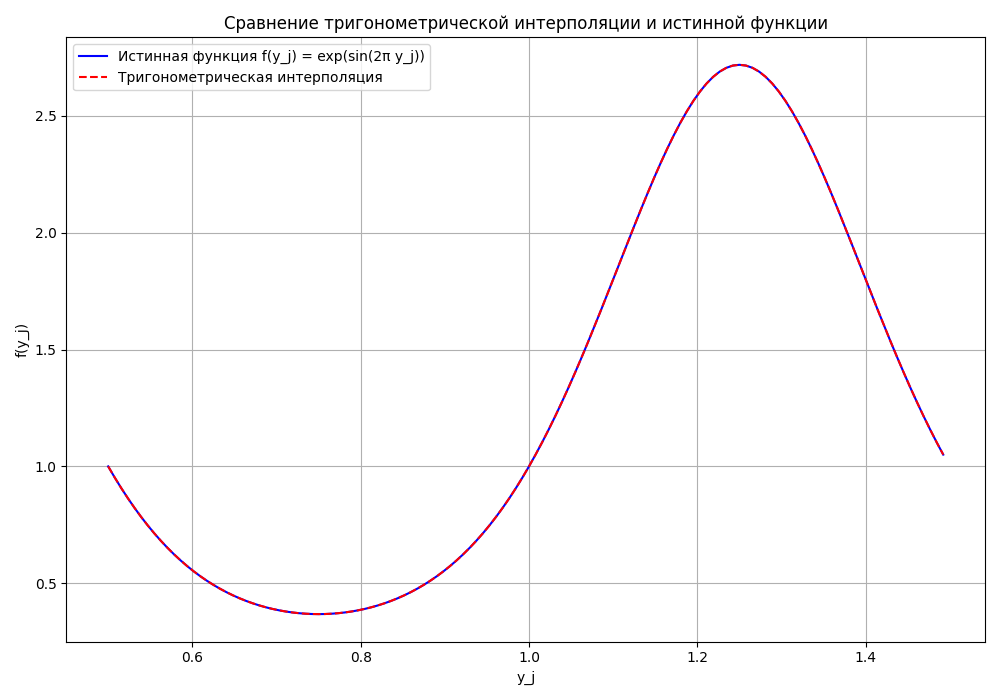
\includegraphics[width=0.8\textwidth]{images/fft.png}
    \caption{График тригонометрической интерполяции и истинной функции \( f(x) = \exp(\sin 2\pi x) \)}
    \label{fig:graph}
\end{figure}


\begin{table}[H]
    \centering
    \caption{Сравнение значений тригонометрической интерполяции и истинных значений в средних точках \( y_j \)}
    \begin{tabular}{ccccc}
    \toprule
    \( j \) & \( y_j \) & Интерполяция & Истинное значение & Абсолютная ошибка \\
    \midrule
    0 & 0.5000 & 1.000000 & 1.000000 & \( 2.48 \times 10^{-15} \) \\
    1 & 0.5078 & 0.952117 & 0.952117 & \( 4.53 \times 10^{-15} \) \\
    2 & 0.5156 & 0.906633 & 0.906633 & \( 4.71 \times 10^{-16} \) \\
    3 & 0.5234 & 0.863527 & 0.863527 & \( 4.09 \times 10^{-15} \) \\
    4 & 0.5312 & 0.822760 & 0.822760 & \( 8.08 \times 10^{-16} \) \\
    5 & 0.5391 & 0.784287 & 0.784287 & \( 3.58 \times 10^{-15} \) \\
    6 & 0.5469 & 0.748051 & 0.748051 & \( 4.22 \times 10^{-15} \) \\
    7 & 0.5547 & 0.713987 & 0.713987 & \( 4.89 \times 10^{-15} \) \\
    8 & 0.5625 & 0.682029 & 0.682029 & \( 6.83 \times 10^{-15} \) \\
    9 & 0.5703 & 0.652101 & 0.652101 & \( 6.54 \times 10^{-15} \) \\
    \bottomrule
    \end{tabular}
\end{table}



\section{Вывод}


В ходе работы успешно реализована тригонометрическая интерполяция функции \( f(x) = \exp(\sin 2\pi x) \) с использованием 
быстрого преобразования Фурье при \( N = 128 \) узлах.
Полученные результаты демонстрируют высокую точность метода - максимальная абсолютная ошибка в средних 
точках составила \( 6.83 \times 10^{-15} \). График визуально показывает совпадение исходной функции и 
интерполянта, что свидетельствует об эффективности тригонометрической интерполяции для точного восстановления значений функции в 
промежуточных точках сетки.

\end{document}